\section{Experimental Data Collection}
 
%Each glider was equipped with a Nortek Signature1000 1 MHz ADCP. Figure \ref{fig.SG} shows an ADCP installed, facing upwards, in the tail section of one of the AUGs. The ADCPs are configured by Nortek to use only three beams---in the upward-facing position, those are the two side beams and the aft beam during descent, and the two side beams and the forward beam during ascent. The ADCPs were programmed to collect a profile every 15 seconds. Each profile covers up to 20 m depth, with a new profile starting approximately every 1.5 m (i.e., the vertical distance covered by the AUG in 15 seconds).
 
 As part of the Canada Basin Glider Experiment (CABAGE), two Seagliders, SG196 and SG198, were deployed on 6 August 2017 at the shelf break north of Prudhoe Bay, AK. From there, they flew up to and around the CANAPE mooring array until they were recovered on 17 September 2017, for a total of 49 days.  Together the gliders covered approximately 1730 km over the course of 712 dives, with SG196 diving to 480 m depth and SG198 diving to 750 m.  Figure \ref{fig:track} shows the glider tracklines for both a short test deployment in 2016 and the 2017 deployment.

\begin{figure}%[!ht]
  \centering
  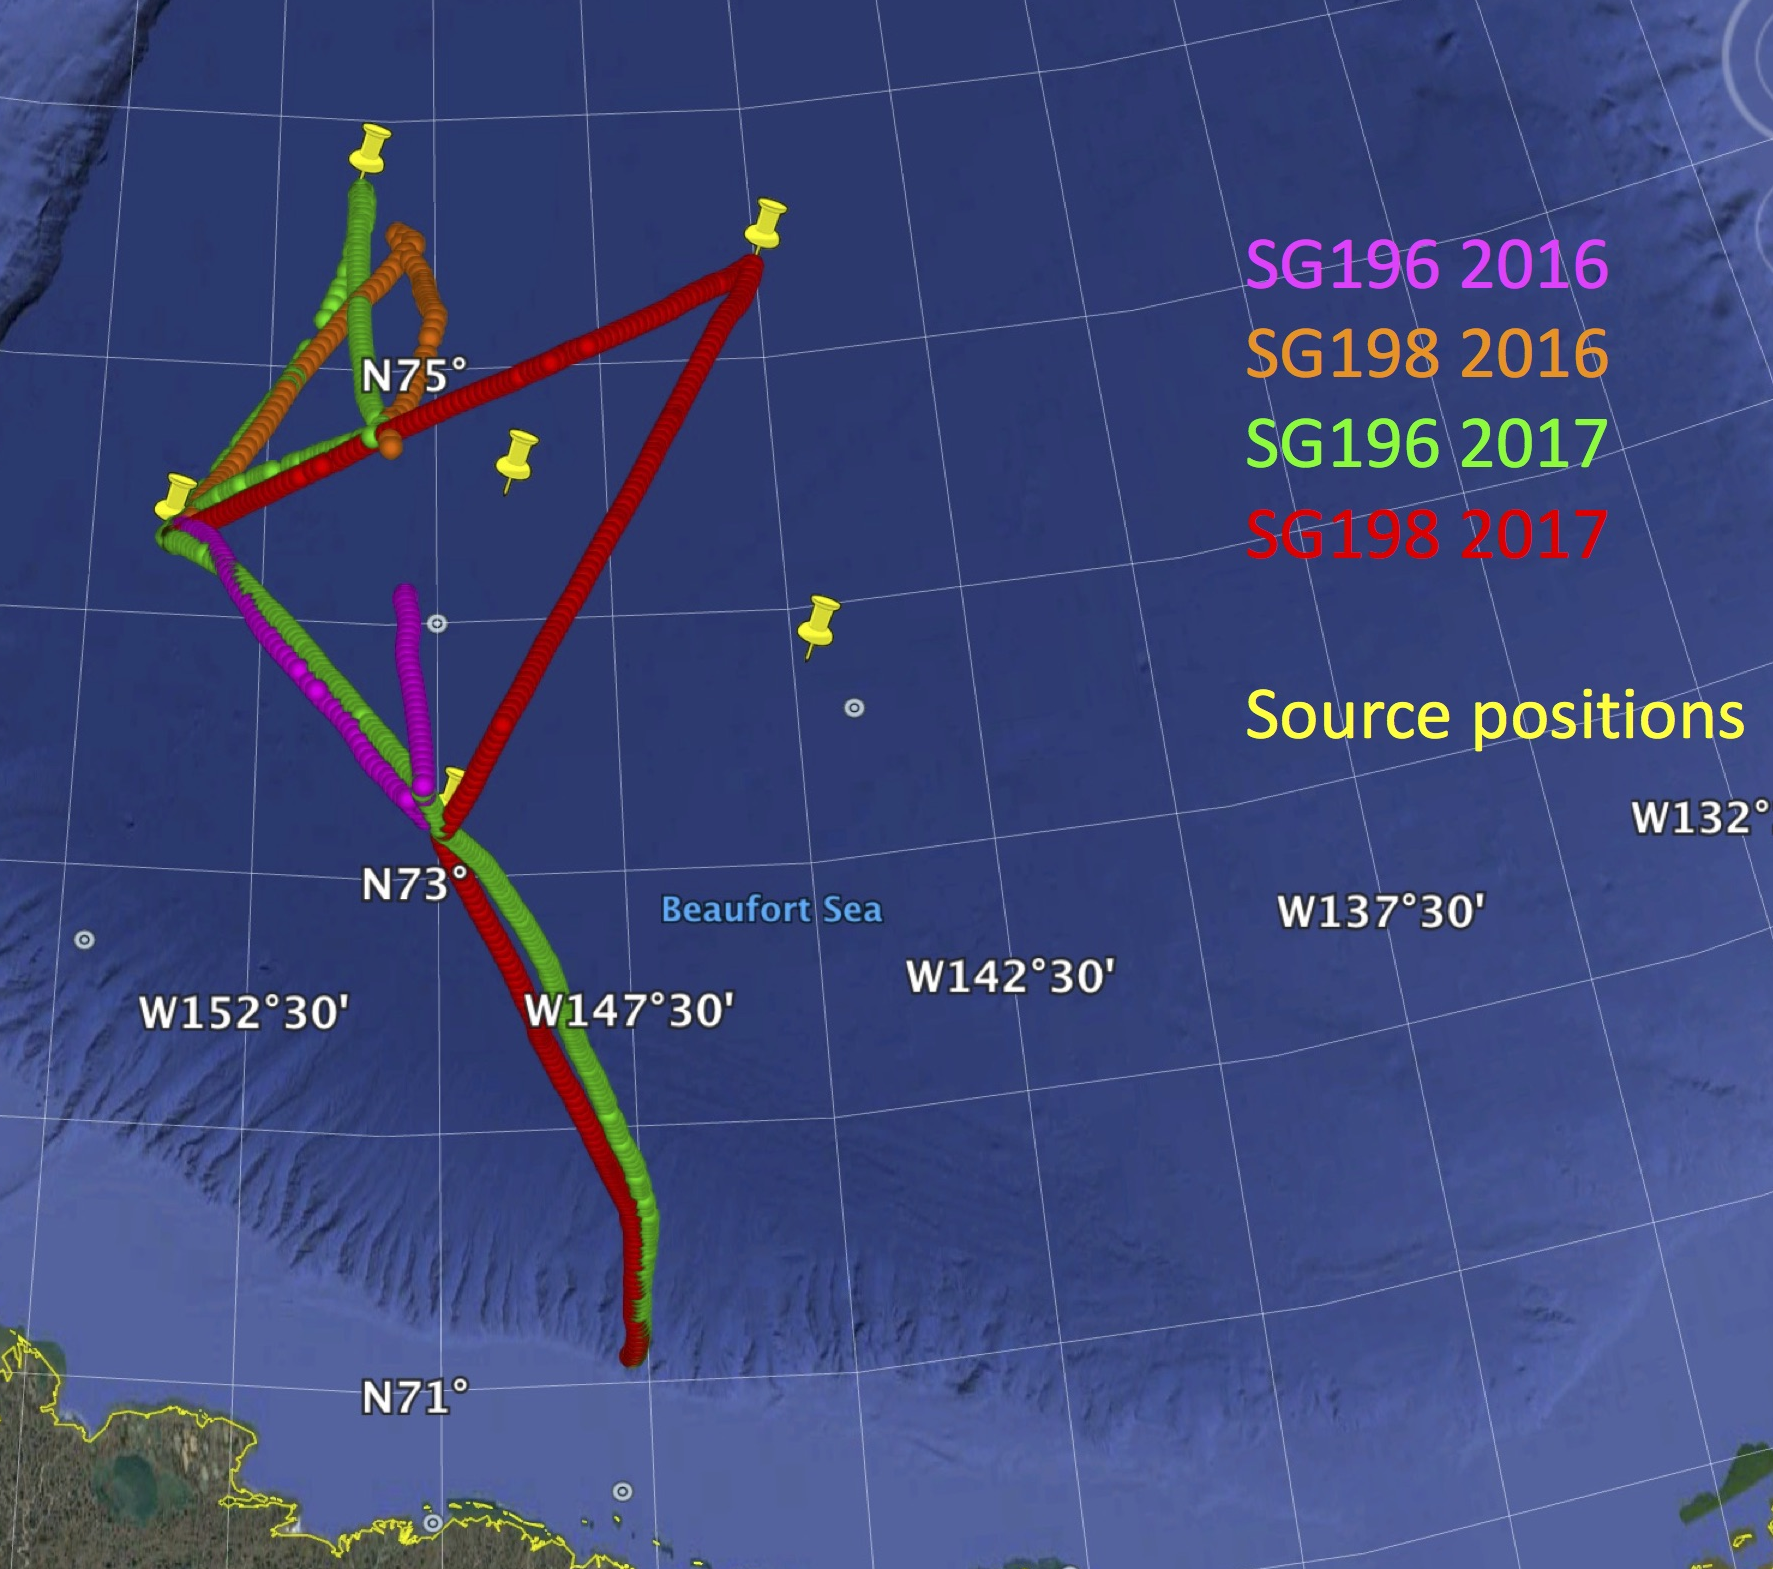
\includegraphics[width=0.9\columnwidth]{./figs/GliderTrajCombined.png}%{./figs/CABAGE_sg198_track_quicklook.png}
  \caption{SG196 and SG198 were deployed at the shelf break north of Prudhoe Bay, AK.  From there, they flew up to and around the CANAPE mooring array until, 49 days later, they were recovered by the USCGC Healy.}
  \label{fig:track}
\end{figure}

Each glider was equipped with a Nortek Signature1000 1 MHz ADCP, as well as the standard suite of conductivity temperature (CT) sensor, pressure sensor, WHOI MicroModem, and custom-built passive marine acoustic recorders (PMARs). Figure \ref{fig:SG} shows the gliders loaded on the R/V Ukpik, ready for launch, with the upward-facing ADCPs, installed in the tail section, clearly visible.

\begin{figure}%[!ht]
  \centering
%  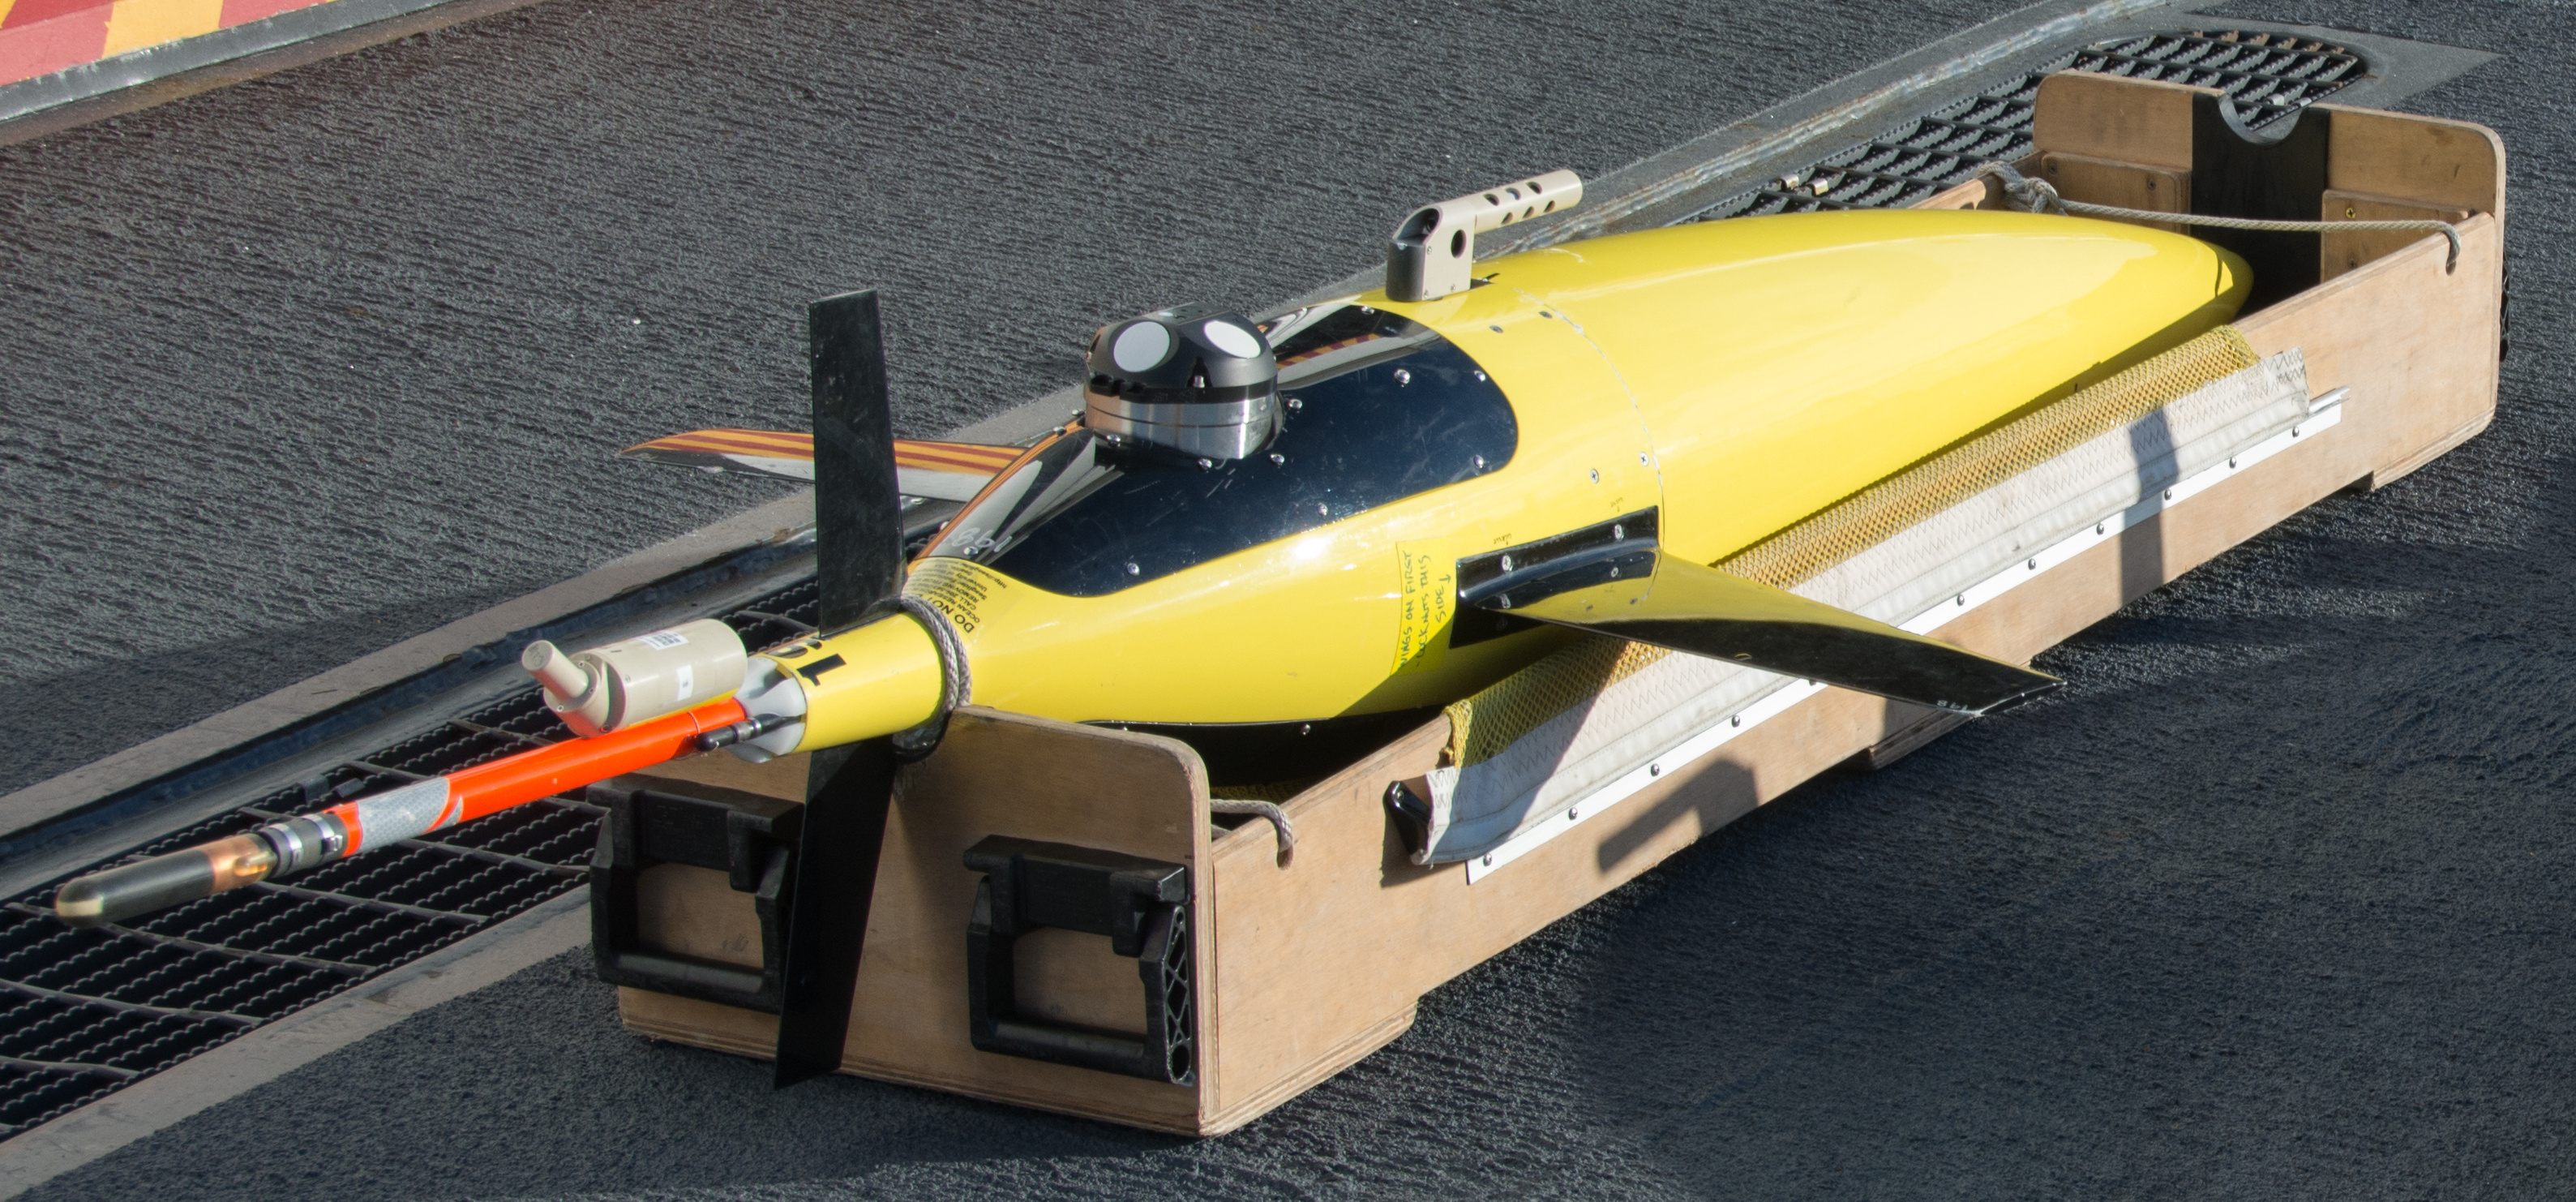
\includegraphics[width=0.6\columnwidth]{./figs/Gliders_hires-99_crop.jpg}
%  \vspace{0.2cm}
  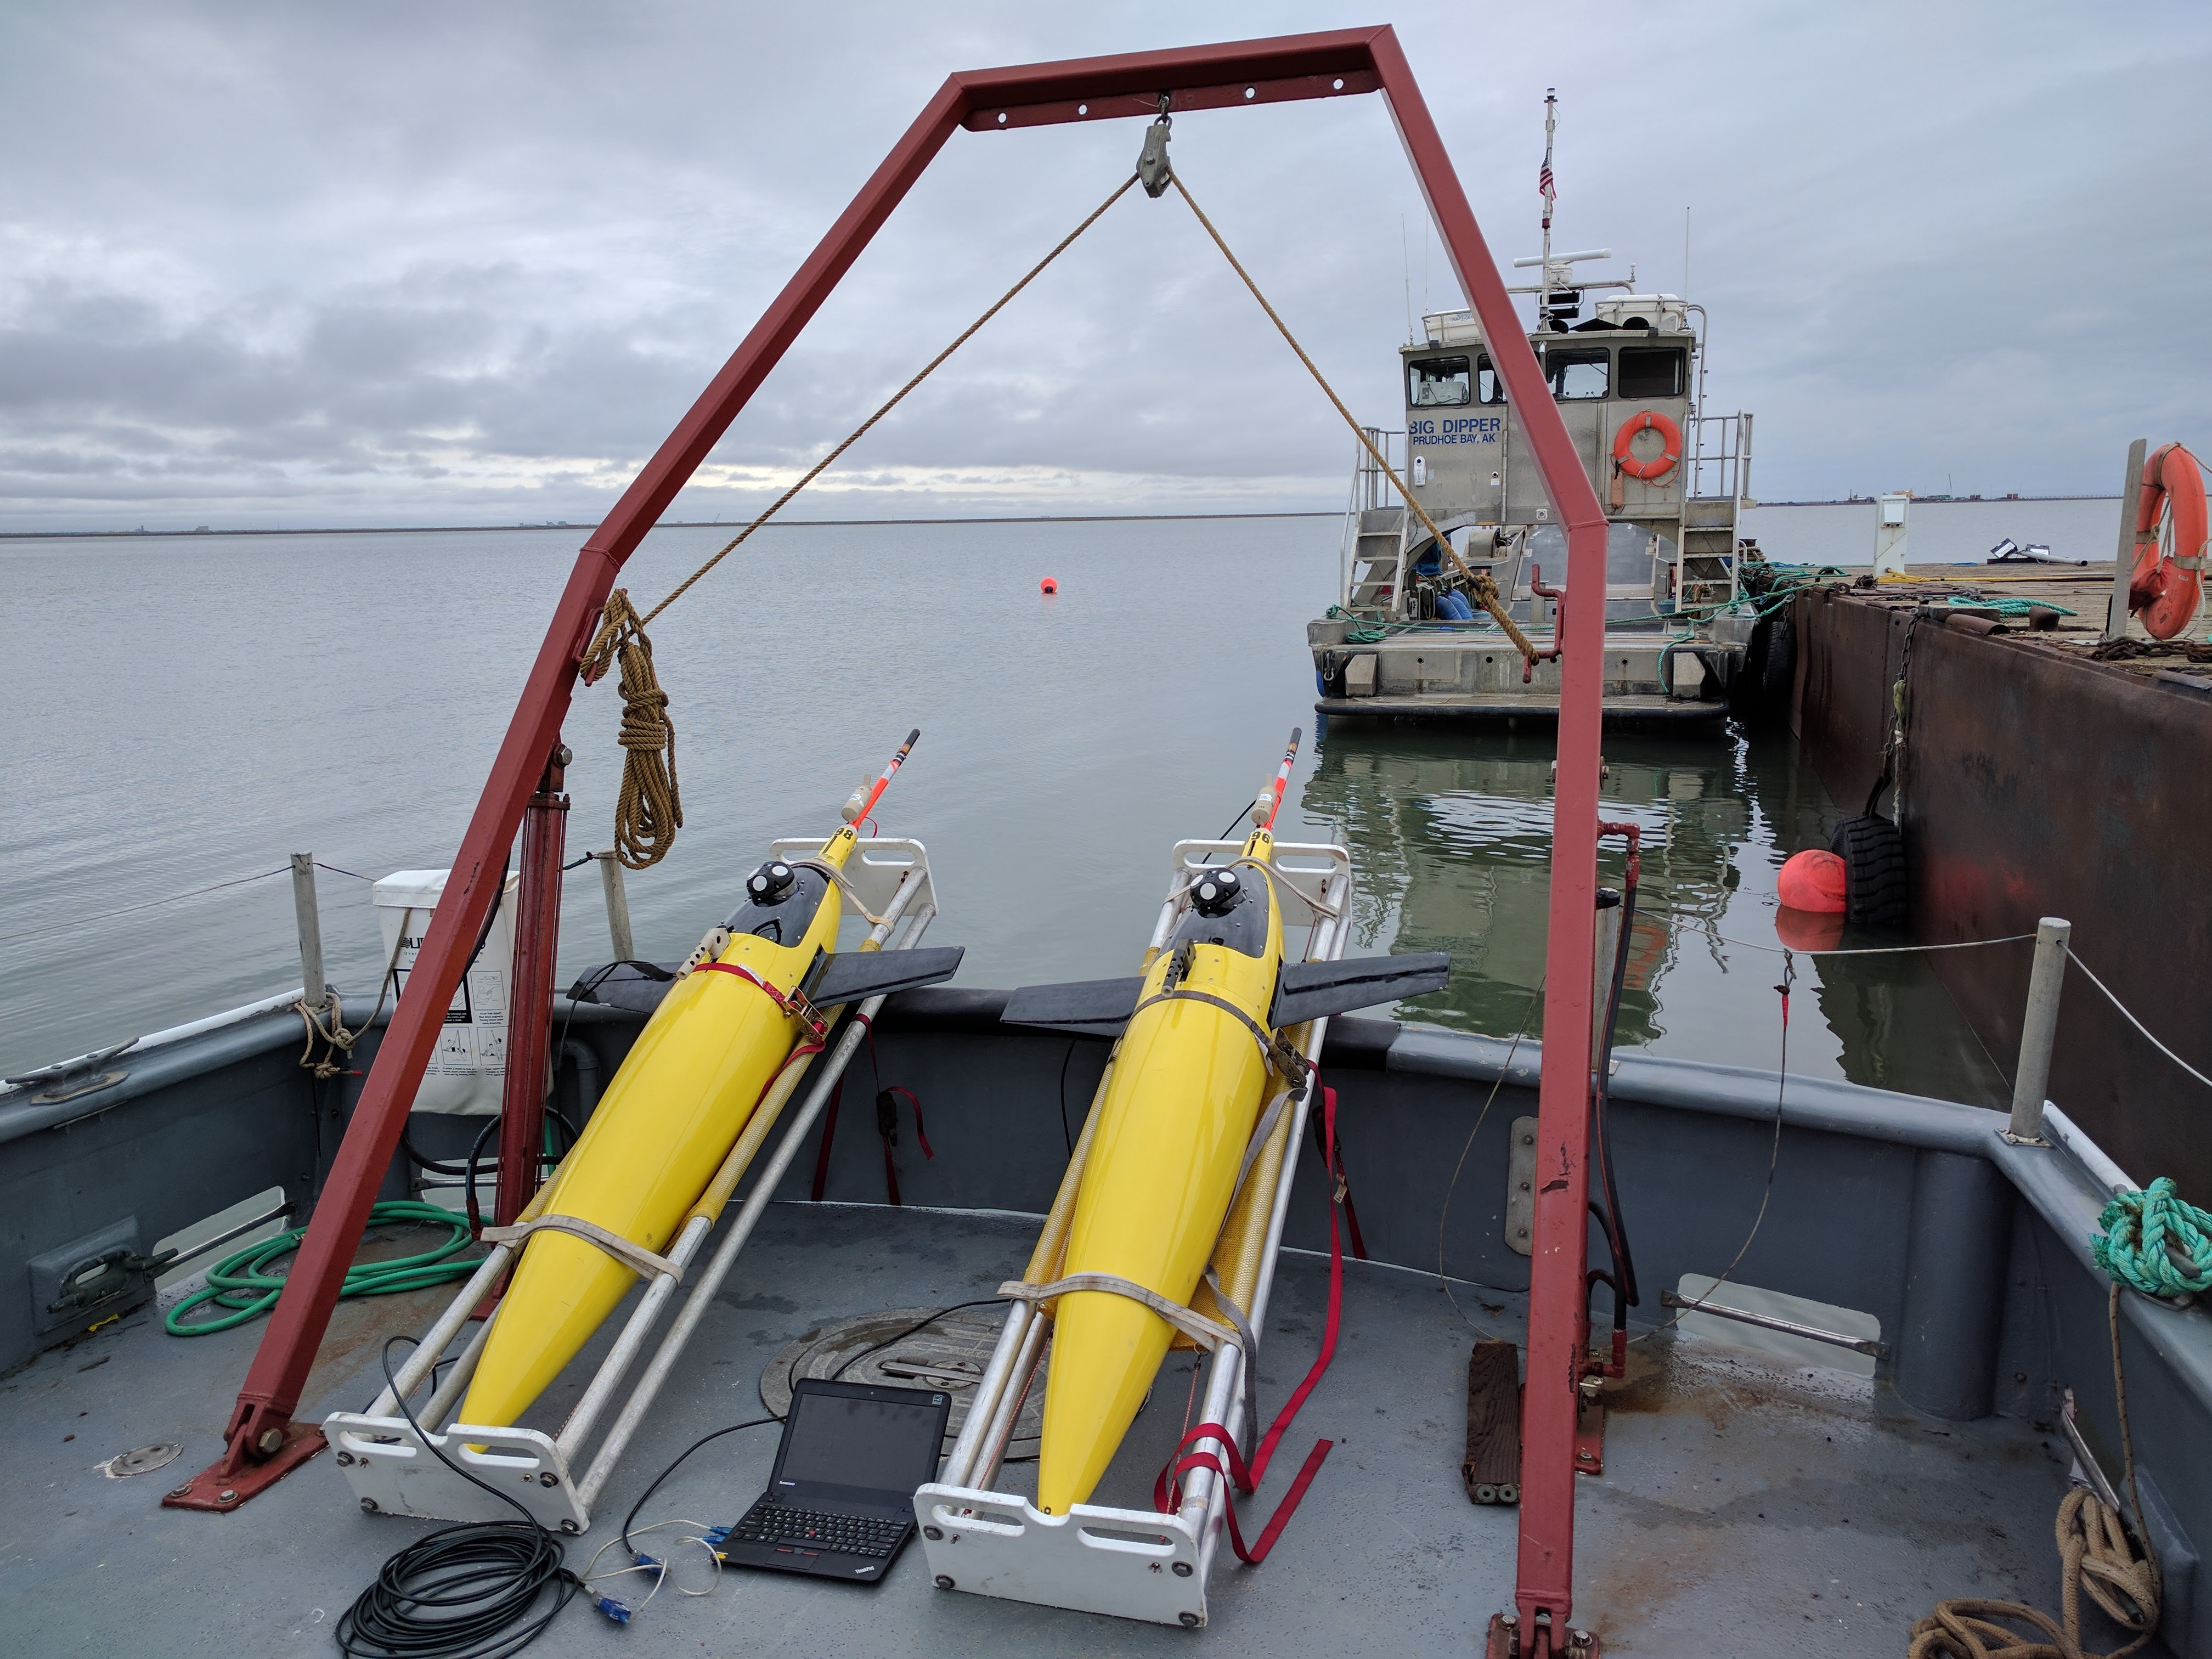
\includegraphics[width=0.9\columnwidth]{./figs/UkpikGliders.jpg}
  \caption{Ready for launch, SG196 and SG198 are loaded on the R/V Ukpik in Prudhoe Bay, AK, with the upward-facing ADCPs, installed in the aft fairing, clearly visible. }
  \label{fig:SG}
  \vspace{-0.2in}
\end{figure}

\begin{figure}%[!ht]
  \centering
  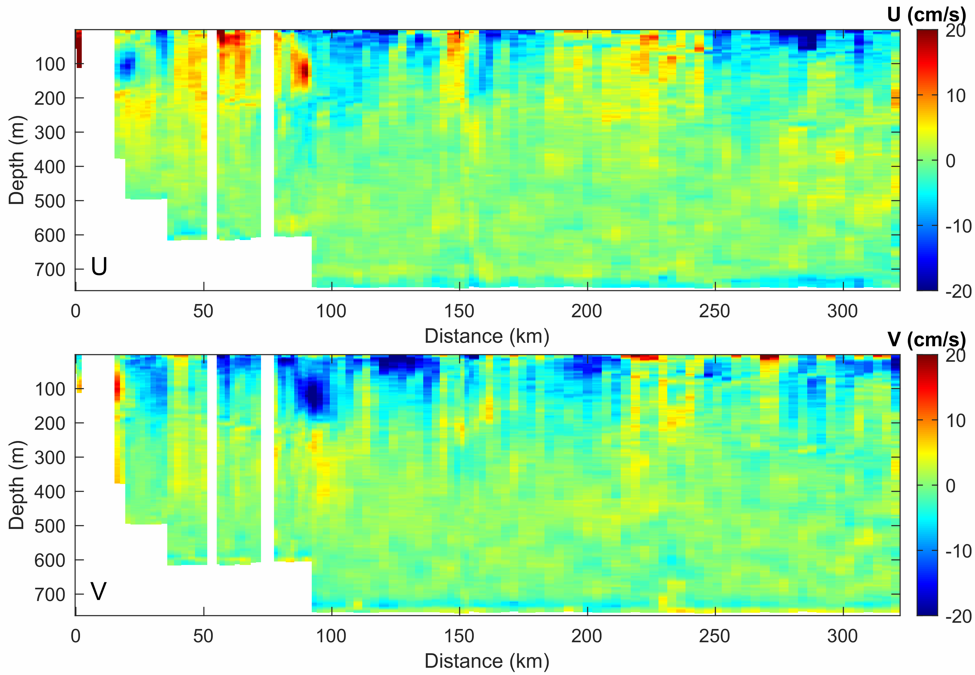
\includegraphics[width=0.9\columnwidth]{./figs/CABAGE_sg198_ADCP_quicklook.png}
  \caption{An example of the cumulative ADCP data collected by SG198 during the first few hundred kilometers of the deployment.}
  \label{fig:ADCP}
\end{figure}

For clarity during the discussion here, when referring to the ADCP data, we will use \emph{trace} to refer to an individual profile collected by the ADCP, and \emph{profile} to refer to the result of the inverse, i.e. the current profile for the entire dive. The ADCPs were programmed to collect a trace every 15 seconds with 2.0 m bins. Each trace typically covered 25m depth, with the actual usable range varying with the amount of acoustic scatterers in the water. As a result, with the typical vertical descent rate of 10 cm/s, any
given depth bin was covered by 15-16 different traces.  Figure \ref{fig:ADCP} illustrates the cumulative ADCP data collected by SG198 during the first few hundred kilometers of the 49-day deployment.
 
%\begin{figure}[!ht]
%  \centering
%  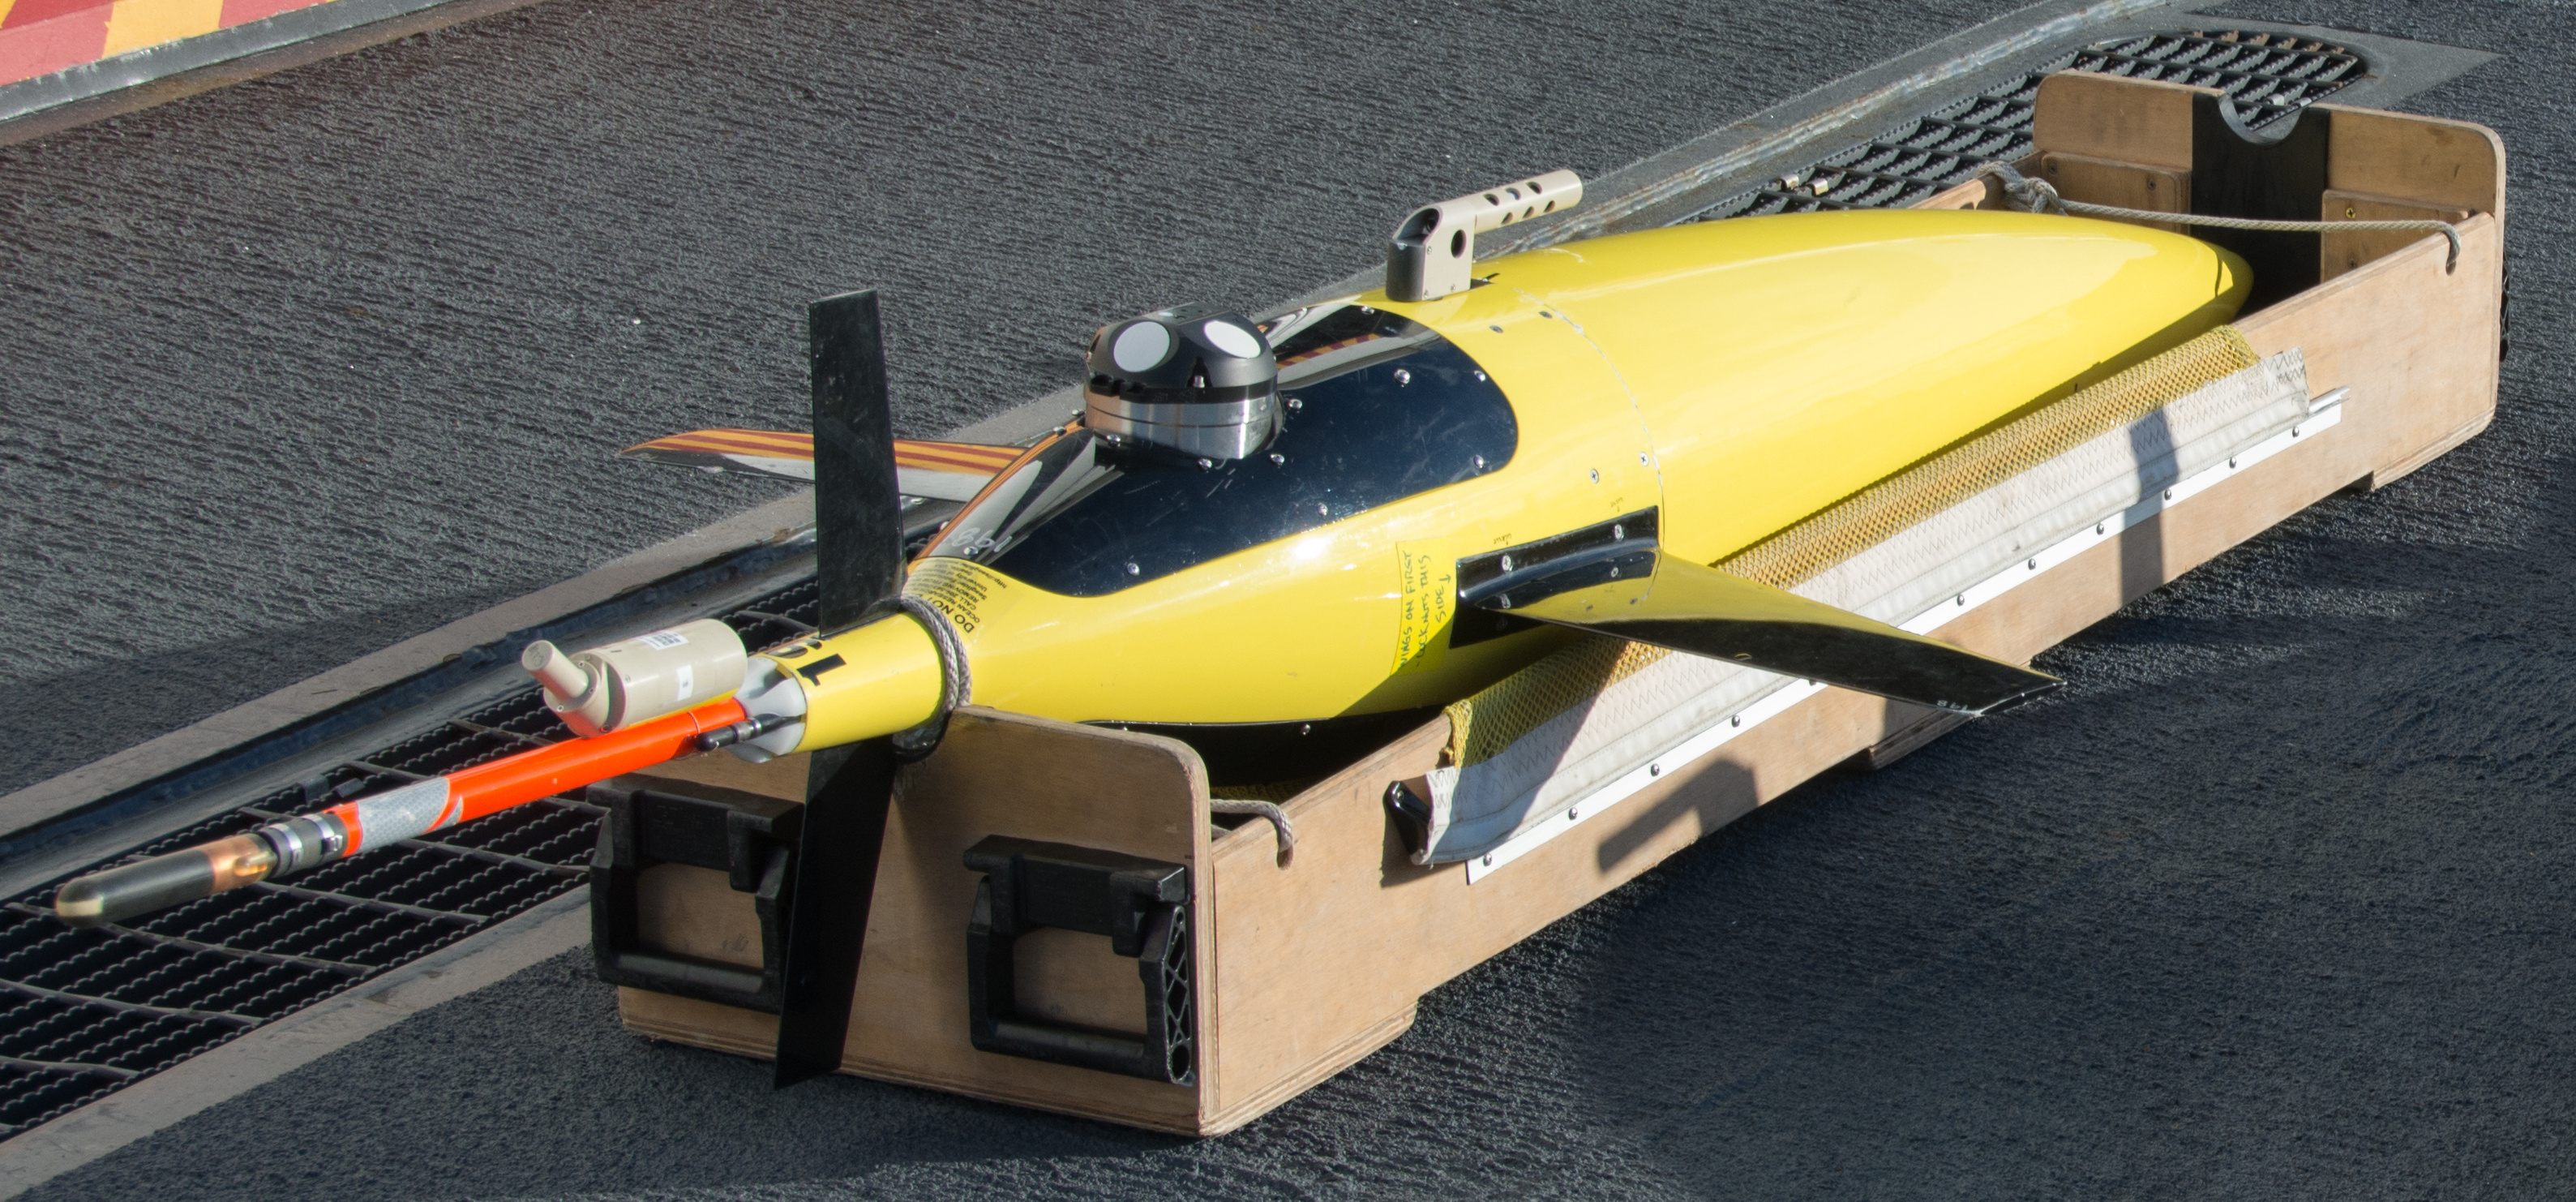
\includegraphics[width=3.0in]{./figs/Gliders_hires-99_crop.jpg}
%  %\vspace{-0.1in}
%  \caption{Seaglider AUG with an upwards-facing ADCP installed in aft %fairing.}
%  \label{fig.SG}
%%   \vspace{-0.1in}
%  %\rule{\textwidth}{0.02in}
%  \vspace{-0.2in}
%\end{figure}
